\chapter{التكاثر اللاجنسي والاستنساخ عند النباتات}\label{ch:b2:asexual-reproduction}

في واد في يوتا تقوم غابة من سبعة وأربعين ألف جذع حور رجراج هي نبات
واحد: فكل جذع نما من الجملة الجذرية نفسها، وكل خلية تحمل المورثوم
نفسه، وعمر الفرد نحو أربعة عشر ألف سنة ووزنه ستة آلاف طن. وكل
فراولة في سلة سوق من صنف واحد قطعة من نبات واحد ضُوعف بالمدادات؛
وكل موزة كافنديش على الأرض عقلة من عقلة من نبات واحد. فالنباتات،
بخلاف معظم الحيوانات، تستطيع صنع أفراد جدد بلا جنس --- من ساق، أو
جذر، أو ورقة، أو خلية واحدة في دورق. يبحث هذا الفصل كيف تفعل ذلك،
وكيف يستغله المزارعون، وما تكلفه السلالةَ مغادرةُ \omterm{def:b2:meiosis-heredity:meiosis}{التقسم المنصّف}
والإلقاح: أي مسألة لماذا يوجد الجنس أصلًا.

\section{التكاثر الخضري}

\begin{definition}[النسيلة والجينيت والراميت]\label{def:b2:asexual-reproduction:clone}
\index{نسيلة}\index{جينيت}\index{راميت}\index{تكاثر خضري}
\emph{التكاثر اللاجنسي} ينتج أفرادًا جددًا من أب واحد بالتقسم
الخيطي وحده، بلا \omterm{def:b2:meiosis-heredity:meiosis}{تقسم منصّف} ولا إلقاح: فالخلف \emph{نسيلة}، مطابقة
وراثيًا للأب وبعضها لبعض، عدا الطفرات الجسدية التي تتراكم. وأشيع
صورها في النباتات \emph{التكاثر الخضري}، حيث يتجذر جزء من
الجسم --- ساق، أو جذر، أو ورقة --- ويصير نباتًا منفصلًا.
و\emph{الجينيت} هو الفرد الوراثي، أي كل ما نما من لاقحة واحدة؛
و\emph{الراميت} وحدة منفصلة فيزيولوجيًا منه. وقد تضم مشتلة فراولة
ألف راميت لجينيت واحد؛ وغابة الحور جينيت واحد. والتكاثر الخضري ممكن
لأن خلايا النبات تحتفظ بالقدرة على الانقسام وتكوين أي عضو ---
فهي \emph{\omterm{prop:b2:asexual-reproduction:tissueculture}{كلية القدرة}} --- ولأن النباتات تنمو من مرستيمات يمكن
إيقاظها في أي موضع تقريبًا.
\end{definition}

\begin{proposition}[أعضاء التكاثر الخضري]\label{prop:b2:asexual-reproduction:organs}
\index{مداد}\index{جذمور}\index{درنة}\index{بصلة}
طوّرت النباتات الحيلة نفسها من كل عضو. فمن السوق: \emph{المدادات}
أو \emph{الجواري}، وهي سوق أفقية على الأرض تتجذر عند عقدها
(الفراولة، والحوذان الزاحف)؛ و\emph{الجذامير}، وهي سوق أفقية تحت
الأرض تتفرع وتتشظى (النجيل، والسوسن، والزنجبيل، \omterm{def:b2:plant-life-cycles:fern}{والسرخس} النسري)؛
و\emph{الدرنات}، وهي أطراف جذامير منتفخة تخزن النشاء وتحمل براعم هي
«العيون» (البطاطا)؛ و\emph{الأكمام}، وهي قواعد سوق عمودية منتفخة
(الزعفران)؛ و\emph{البصيلات}، وهي بصلات صغيرة تتكون في آباط الأوراق
أو في النورة (الثوم، وبعض أنواع البصل). ومن الأوراق: \emph{البصلات}،
وهي براعم ملفوفة في أوراق تخزين لحمية تنشطر إلى بصلات بنات
(البصل، والخزامى)؛ ونبيتات على حافة الورقة، كاملة بجذورها، تسقط
(\emph{Kalanchoe}). ومن الجذور: \emph{الخلفات}، وهي سوق تنهض من
جذور أفقية (الحور الرجراج، والبرقوق البري، والتوت الشوكي). وبطريق
\emph{التشظي}: قطعة غصن صفصاف تطفو بعيدًا فتتجذر، وسعفة عدس ماء
تنشطر. وفي كل حالة يُحمل عضو تخزين أو مرستيم مسافة قصيرة، وتبدأ
البنت حياتها بمؤونة غذاء لا تضاهيها \omterm{def:b2:angiosperm-reproduction:seed}{بذرة}.
\end{proposition}

\begin{omfigure}
\begin{tikzpicture}[every node/.style={font=\scriptsize}]
  % runner
  \begin{scope}
    \draw[thick] (0,0) -- (3.6,0);
    \foreach \x in {0,1.8} { \draw[thick, omExo!70!black, fill=omExo!30] (\x,0) .. controls (\x-0.3,0.6) and (\x+0.3,0.6) .. (\x,0); \foreach \a in {60,90,120} \draw[thick, omExo!70!black] (\x,0) -- ++(\a:0.7); \draw[gray] (\x,0) -- ++(-100:0.4) (\x,0) -- ++(-70:0.4); }
    \draw[thick, omThm] (0.2,0.15) .. controls (0.9,0.55) and (1.2,0.55) .. (1.8,0.1);
    \draw[thick, omThm] (2.0,0.15) .. controls (2.7,0.55) and (3.0,0.55) .. (3.5,0.1);
    \draw[thick, omExo!70!black] (3.5,0.1) -- ++(80:0.4); \draw[gray] (3.5,0.1) -- ++(-80:0.3);
    \node[below, align=center] at (1.8,-0.55) {مداد (الفراولة):\\ساق أفقية تتجذر عند عقدها};
  \end{scope}
  % rhizome and tuber
  \begin{scope}[xshift=5.2cm]
    \draw[gray, dashed] (-0.2,0) -- (3.8,0);
    \draw[very thick, omProp!80!black] (0,-0.5) -- (3.4,-0.5);
    \foreach \x in {0.6,2.0} \draw[thick, omExo!70!black] (\x,-0.5) -- (\x,0.7) (\x,0.3) -- ++(40:0.4) (\x,0.3) -- ++(140:0.4);
    \draw[thick, omProp!80!black, fill=omProp!40] (3.4,-0.5) ellipse (0.45 and 0.3);
    \foreach \p in {(3.2,-0.3),(3.6,-0.35),(3.7,-0.6)} \fill[omThm] \p circle (0.04);
    \foreach \x in {0.3,1.3,2.5} \draw[gray] (\x,-0.5) -- (\x,-0.9);
    \node[below, align=center] at (1.8,-1.05) {جذمور ودرنة (البطاطا):\\سوق تحت الأرض،\\وبراعم (عيون) على الدرنة};
  \end{scope}
  % bulb
  \begin{scope}[xshift=12.2cm]
    \draw[thick, fill=omExo!15] (0,-0.9) .. controls (-0.9,-0.6) and (-0.9,0.9) .. (0,1.0) .. controls (0.9,0.9) and (0.9,-0.6) .. (0,-0.9);
    \foreach \r in {0.55,0.35} \draw[thick] (0,-0.75) .. controls (-\r,-0.5) and (-\r,0.6) .. (0,0.8) .. controls (\r,0.6) and (\r,-0.5) .. (0,-0.75);
    \fill[omExo!60!black] (-0.1,-0.75) rectangle (0.1,0.3);
    \draw[thick, omThm, fill=omThm!30] (0.35,-0.5) ellipse (0.15 and 0.3);
    \foreach \x in {-0.3,0,0.3} \draw[gray] (\x,-0.9) -- (\x,-1.25);
    \node[below, align=center] at (0,-1.3) {بصلة (البصل):\\أوراق لحمية،\\وبصلة بنت (بالأحمر)};
  \end{scope}
\end{tikzpicture}

{\small ثلاثة أعضاء \omterm{def:b2:asexual-reproduction:clone}{للتكاثر الخضري}: مدادات تتجذر عند عقدها، وساق
تحت الأرض تنتفخ درنةً، وبصلة \omterm{def:b2:unicellular-diversity:division}{تبرعم} بصلة بنتًا. وفي كل حالة يسافر
برعم ومعه غذاؤه.}
\end{omfigure}

\begin{omfigure}
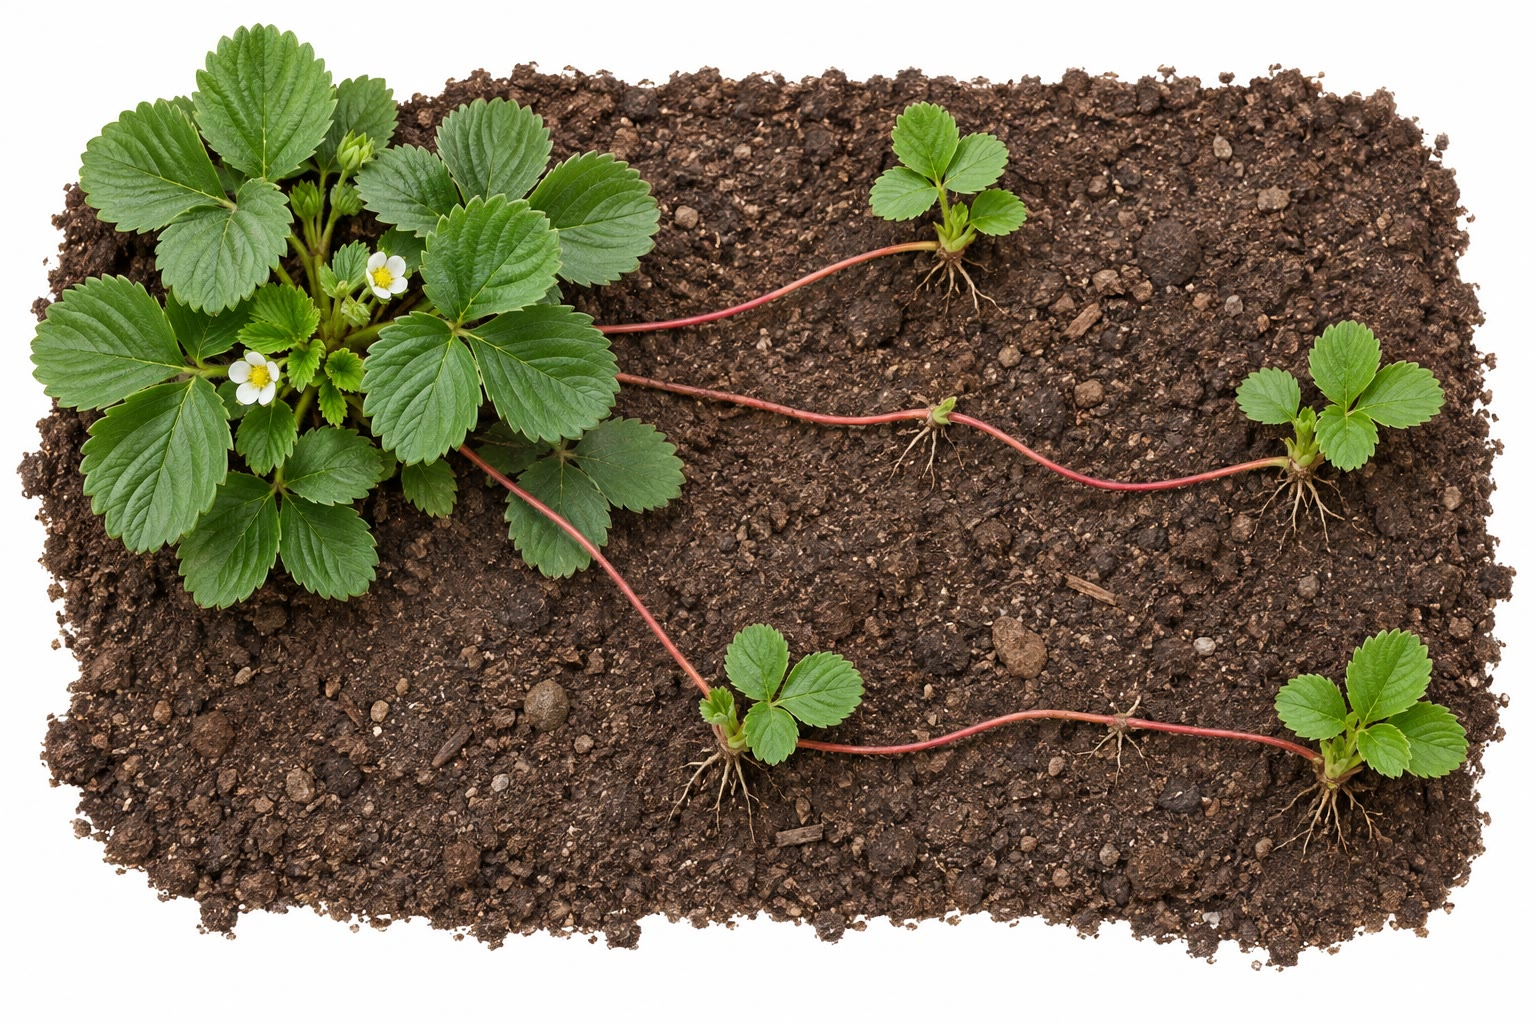
\includegraphics[width=0.46\linewidth]{images/book4/ai/b4-07-strawberry-runners.jpg}\hspace{0.03\linewidth}
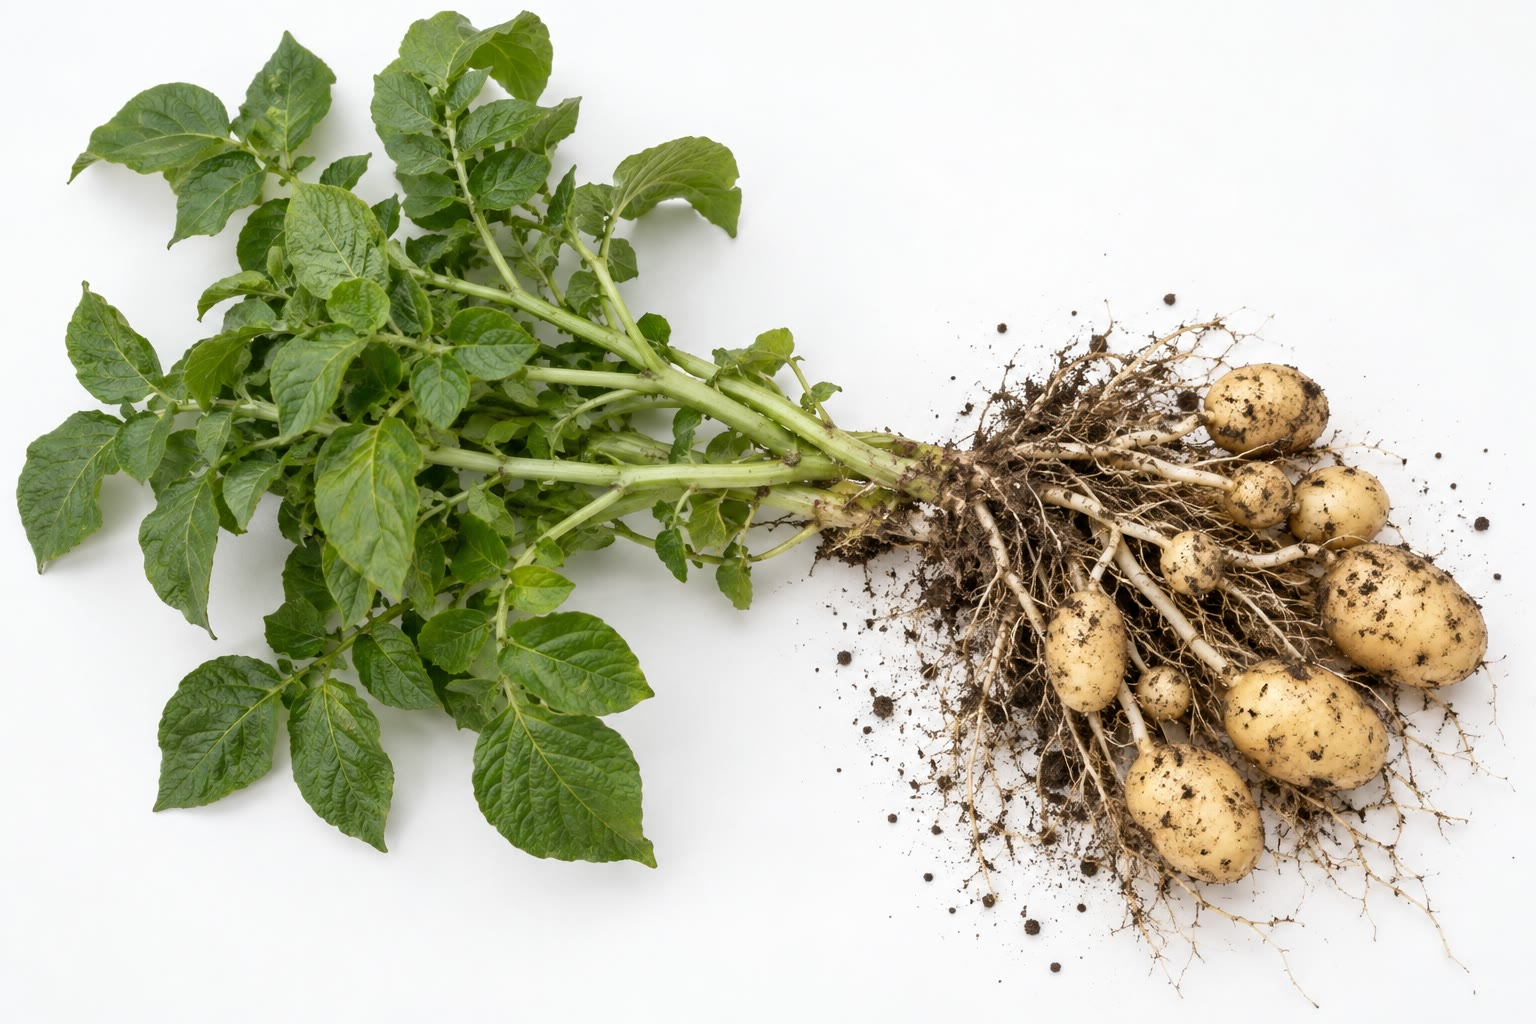
\includegraphics[width=0.46\linewidth]{images/book4/ai/b4-07-potato-tubers.jpg}

{\small على اليمين: نبات فراولة والنباتات البنات المتجذرة على
امتداد مداداته. وعلى اليسار: نبات بطاطا مرفوع من التربة، ودرناته
معلقة على جوارٍ --- وكل درنة قطعة ساق ستنمو نباتًا مطابقًا وراثيًا
لهذا.}
\end{omfigure}

\begin{theorem}[هندسة نسيلة منتشرة]\label{thm:b2:asexual-reproduction:spread}
\index{نمو نسيلي}
\omterm{def:b2:asexual-reproduction:clone}{جينيت} ينتج كل \omterm{def:b2:asexual-reproduction:clone}{راميت} فيه $m$ بنتًا متجذرة في السنة، وتبقى كلها،
ينمو عددًا وفق $N(t) = N_0 (1 + m)^t$ --- أي نموًا أسّيًا بلا أي
جنس --- إلى أن تملأ الراميتات المكان عند كثافة حمولتها $d$
(\omterm{def:b2:asexual-reproduction:clone}{راميت} في وحدة المساحة)، فتتقدم \omterm{def:b2:asexual-reproduction:clone}{النسيلة} بعد ذلك جبهةً. \omterm{def:b2:asexual-reproduction:clone}{والنسيلة}
التي تمد مداداتها في خط مستقيم بسرعة $v$ يكون نصف قطرها بعد $t$
سنة مقداره $vt$، وينمو عدد الراميتات وفق $\pi d (vt)^2$: أي
تربيعيًا لا أسّيًا. فنبات فراولة يرسل مداداته \qty{0.5}{m} في السنة
يكون نصف قطره \qty{5}{m} بعد عشر سنوات؛ \omterm{def:b2:asexual-reproduction:clone}{ونسيلة} الحور في الفقرة
الافتتاحية، ومساحتها \qty{43}{ha}، نصف قطرها نحو \qty{370}{m}، وعند تقدم صافٍ قدره بضعة سنتيمترات في السنة يكون
عمرها من رتبة $10^{4}$ سنة --- وهو متسق مع العمر المقدَّر
من انحسار الجليديات.
\end{theorem}
\begin{proof}
يُستبدل بكل \omterm{def:b2:asexual-reproduction:clone}{راميت} في كل سنة هو نفسه زائد $m$ بنتًا، أي بعامل
$1 + m$؛ فتعطي $t$ سنة عامل $(1 + m)^t$. وحين يمتلئ الداخل، لا تجد
مكانًا إلا الراميتات على الحافة، وتتقدم الحافة
بسرعة المدادات $v$؛ فتكون المساحة $\pi(vt)^2$ ويكون عدد
الراميتات المساحة مضروبة في الكثافة.
\end{proof}

\begin{example}[أقدم الكائنات]\label{ex:b2:asexual-reproduction:oldest}
تغطي \omterm{def:b2:asexual-reproduction:clone}{نسيلة} الحور المسماة باندو (يوتا) \qty{43}{ha} بنحو
\num{47000} جذع يعيش كل منها قرنًا أو نحوه ويُستبدل به
خلفات من الجذور نفسها؛ وقد يزيد عمر \omterm{def:b2:asexual-reproduction:clone}{الجينيت} على عشرة آلاف
سنة. \omterm{def:b2:asexual-reproduction:clone}{ونسيلة} من عشب البحر \emph{Posidonia} في
المتوسط تمتد \qty{15}{km} وقد يبلغ عمرها مئة ألف
سنة؛ وحلقة من شجيرات الكريوزوت في موهافي أُرّخت إلى
\num{11700} سنة، وسوقها المركزية تموت والحلقة تتسع. وفي
كل حالة يكون القديم هو \omterm{def:b2:asexual-reproduction:clone}{الجينيت}؛ ولا خلية فيه أقدم من
بضعة عقود، وقد نُسخ المورثوم آلاف المرات.
\end{example}

\section{بذور بلا جنس، وحيوانات بلا آباء}

\begin{definition}[التوالد العذري البذري]\label{def:b2:asexual-reproduction:apomixis}
\index{توالد عذري بذري}\index{توالد عذري}
\emph{التوالد العذري البذري} إنتاج بذور بلا إلقاح: إذ ينمو جنين من
بويضة غير مختزلة (فتتخطى خلية أم \omterm{def:b2:plant-life-cycles:heterospory}{البوغ الكبير} \omterm{def:b2:meiosis-heredity:meiosis}{التقسم المنصّف}) أو
ينمو مباشرة من خلية من النوسيلة، فتحمل \omterm{def:b2:angiosperm-reproduction:seed}{البذرة} \omterm{def:b2:meiosis-heredity:vocabulary}{النمط الوراثي} للأم.
والهندباء، والنَّتِنة، والتوت الشوكي، ودرن مروج كنتاكي وكثير من
الحمضيات تفعل هذا؛ \omterm{def:b2:angiosperm-reproduction:seed}{وبذرة} الحمضيات كثيرًا ما تحوي عدة أجنة، واحد
جنسي والبقية نسخ نوسيلية من الأم. والتوالد العذري البذري يبقي
\omterm{def:b2:angiosperm-reproduction:seed}{البذرة} --- بانتشارها وسكونها وقشرتها --- ويسقط \omterm{def:b2:meiosis-heredity:meiosis}{التقسم المنصّف}، فيُبث
\omterm{def:b2:meiosis-heredity:vocabulary}{نمط وراثي} حسن التكيف من غير تغيير؛ ومعظم المتوالدات عذريًا متعددات
صيغة من أصل هجين كان تقسمها المنصّف ليفشل على كل حال. ونظير ذلك عند
الحيوان هو \emph{التوالد العذري}، أي النمو من بويضة غير ملقحة:
وهو إلزامي عند بعض السحالي وعند الدولابيات البدلوئيدية التي لم يكن
لها ذكور منذ عشرات ملايين السنين؛ ودوري عند المنّ وبراغيث الماء،
التي تتكاثر عذريًا طوال الصيف، فتلد الأنثى بنات حيات يحملن أجنتهن
سلفًا، ثم تتحول في الخريف إلى جيل جنسي يضع بيضًا يشتّي.
\end{definition}

\begin{omfigure}
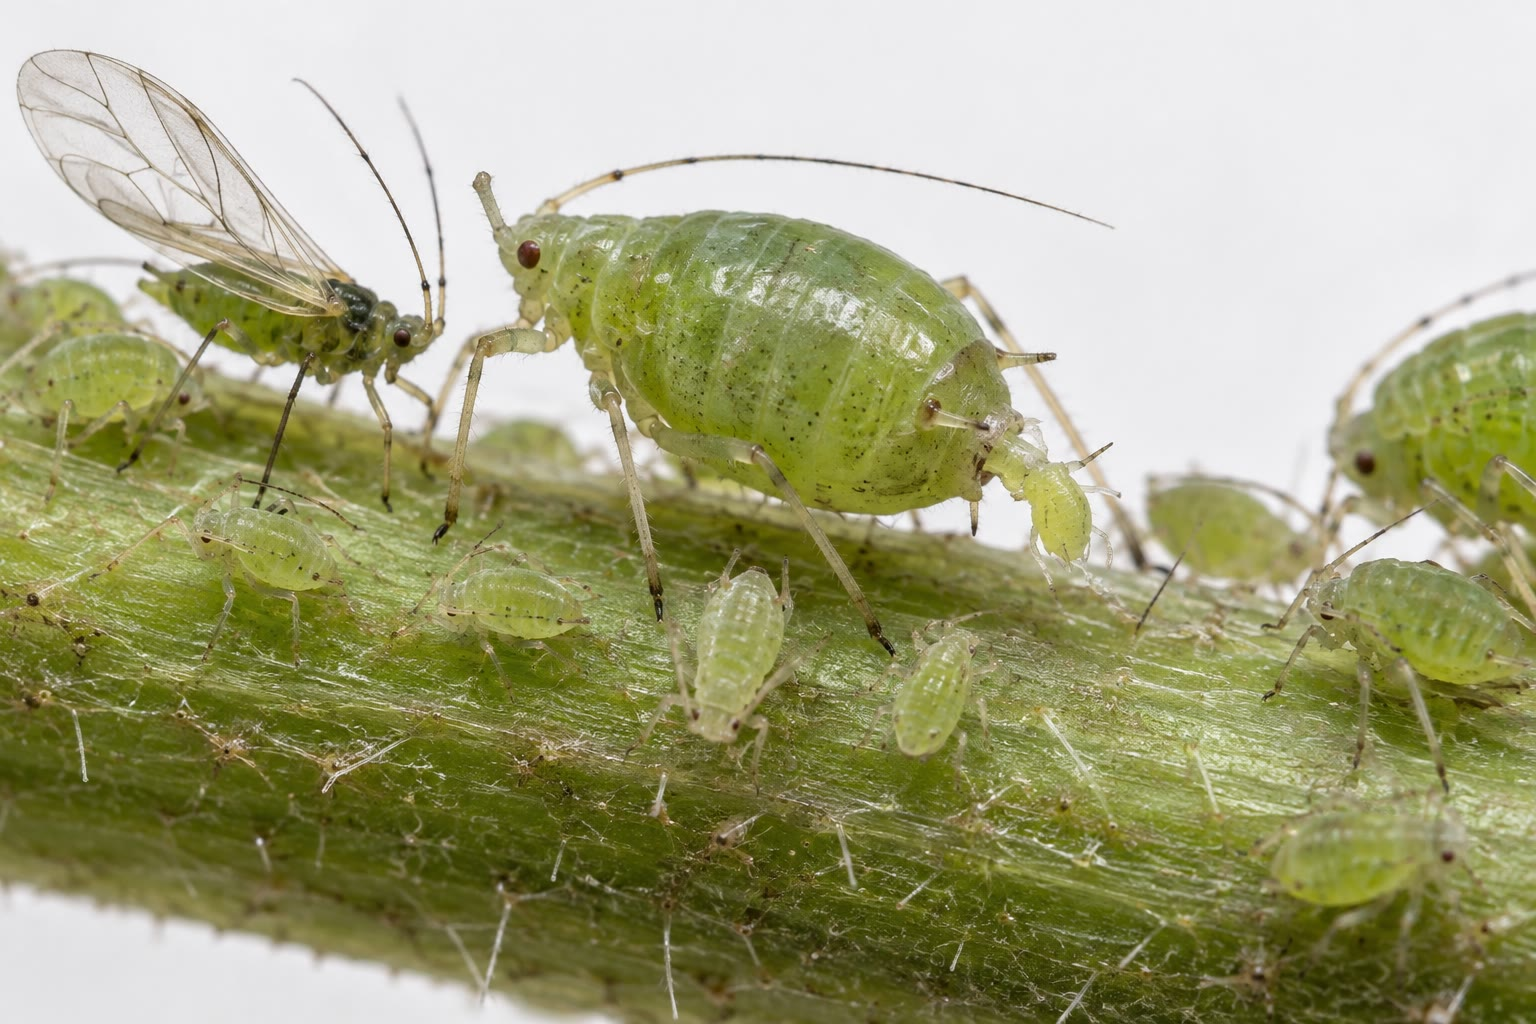
\includegraphics[width=0.55\linewidth]{images/book4/ai/b4-07-aphids.jpg}

{\small منّ على ساق: أنثى عذرية بلا أجنحة تلد بنتًا حية، وحوريات من
أعمار عدة، ومهاجرة مجنحة --- أي نمو أسّي طوال صيف بلا ذكر واحد.}
\end{omfigure}

\begin{example}[صيف من المنّ]\label{ex:b2:asexual-reproduction:aphids}
تنضج منّة عذرية في نحو ثمانية أيام وتنتج
نحو خمس بنات في اليوم على مدى أسبوعين؛ وتولد البنات حوامل
سلفًا (إذ تبدأ الأجنة بالنمو داخل أجنة الأم). ومع زمن جيل قريب من
عشرة أيام ومعدل زيادة صافٍ قدره نحو \num{50} في الجيل، تستطيع
مؤسِّسة واحدة في نيسان، لو تُركت، أن تخلّف $50^{12} \approx 2\times 10^{20}$
خلفًا في غضون أربعة أشهر --- أي أكثر كتلةً من كل حيوان حي اليوم. لكن
الدعاسيق، وأسود المنّ، والزنابير المتطفلة، والفطريات، والمطر تبقي
العدد عند بضعة آلاف في النبات، ويعيد الجيل الجنسي الخريفي ضبط
\omterm{def:b2:asexual-reproduction:clone}{النسيلة} في بيوض معادة التركيب قبل الشتاء.
\end{example}

\section{الاستنساخ عند المزارع}

\begin{proposition}[العقل والترقيد والتطعيم]\label{prop:b2:asexual-reproduction:horticulture}
\index{عقلة}\index{تطعيم}\index{أصل}
\emph{العقلة} قطعة ساق أو جذر أو ورقة تُستحث على التجذر:
فيكوّن الطرف المقطوع دشبذًا من خلايا منقسمة تنشأ منه مرستيمات
جذرية، يساعدها الأوكسين (هرمون التجذير) والرطوبة.
و\emph{الترقيد} يجذّر غصنًا وهو لا يزال متصلًا ثم يقطعه
بعد ذلك. و\emph{التطعيم} يصل فرعًا من نبات (وهو
\emph{الطُّعم}) بالساق المتجذرة لنبات آخر (وهو \emph{الأصل}):
إذ يُضغط الكامبيومان أحدهما على الآخر، ويجسر الدشبذ الجرح، ويصل
خشب ولحاء جديدان عبره في غضون أسابيع. والطُّعم شيمرا
--- فالجذور تبقي مورثوم الأصل، والفرع المثمر مورثوم
الطُّعم --- ولا ينجح إلا بين نباتات قريبة (أنواع من جنس واحد،
وأحيانًا من فصيلة واحدة)، لأن على الأنسجة أن تتعارف
خلاياها. وكل صنف من التفاح والكمثرى والكرز والحمضيات
والعنب يُكاثر بالتطعيم: فالصنف المسمّى \omterm{def:b2:asexual-reproduction:clone}{جينيت} واحد،
أُبقي حيًا قرونًا بالطُّعوم (فتفاح الرينيت يعود
إلى القرن السادس عشر)، ويُختار الأصل بحسب
التربة والمرض وقياس الشجرة المطلوب --- فالأصول
المقزّمة تصنع الأشجار الصغيرة في البساتين الحديثة.
\end{proposition}

\begin{proposition}[التكاثر المجهري وكلية القدرة]\label{prop:b2:asexual-reproduction:tissueculture}
\index{تكاثر مجهري}\index{كلية القدرة}\index{دشبذ}
كل خلية نباتية حية ذات نواة تستطيع، من حيث المبدأ، أن تجدد نباتًا
كاملًا. ففي \emph{زرع الأنسجة} توضع قطعة نسيج معقّمة
(\emph{مستنبت}: قمة فرع، أو قرص ورقة، أو متك) على وسط
من الآغار فيه سكر ومعادن وفيتامينات وهرمونات. فمع توازن
الأوكسين والسيتوكينين تتنزع خلايا التمايز فتصير
\emph{دشبذًا}، وهو كتلة من خلايا منقسمة غير متخصصة؛ ومع
سيتوكينين أكثر من الأوكسين يكوّن الدشبذ فروعًا، ومع أوكسين أكثر من
السيتوكينين يكوّن جذورًا، وفي بعض الأنواع يكوّن \emph{أجنة
جسدية} --- أي أجنة كاملة بلا بويضة. وتُقطع الفروع
وتُعاد زراعتها كل بضعة أسابيع، فتتضاعف بعامل ثلاثة إلى
عشرة في كل مرة، حتى يعطي مرستيم واحد مليون نبيتة في
سنة. ولأن الفيروسات تتخلف عن القمة النامية، تكون قمة فرع
مرستيمية أقصر من مليمتر خالية من الفيروس عادةً حتى في نبات
مصاب: وإنما \emph{زرع المرستيم} هو الطريق الذي تُنقّى به
سلالات البطاطا والفراولة والموز والسحلبيات. والطريقة هي
البرهان العملي على \omterm{prop:b2:asexual-reproduction:tissueculture}{كلية القدرة}، وسبب إمكان بيع صنف نباتي
بالملايين في غضون سنوات قليلة من إنشائه.
\end{proposition}
\begin{proof}[شواهد]
نمّى سكوغ وميلر (1957) دشبذًا من نخاع التبغ على أوساط بنسب مختلفة
من الأوكسين إلى السيتوكينين المكتشف حديثًا: فأعطى الأوكسين المرتفع
جذورًا، وأعطى السيتوكينين المرتفع فروعًا، وأعطى التوازن دشبذًا
فقط --- فتكوين الأعضاء تضبطه نسبة هرمونين، لا مادة
خاصة مكوّنة للأعضاء. وعلّق ستيوارد (1958) خلايا مفردة وكتلًا صغيرة
من جذر جزر في دورق دوّار فيه حليب جوز الهند: فكوّنت بعض الكتل بنى
شبيهة بالأجنة نمت جزرًا مزهرًا كاملًا، وهو ما بيّن أن خلية متمايزة
من عضو ناضج لا تزال تحمل برنامج النمو كله وتستطيع استعماله.
\end{proof}

\begin{omfigure}
\begin{tikzpicture}[every node/.style={font=\scriptsize}, >=stealth]
  \node[draw, rounded corners, fill=omDef!12, align=center] (ex) at (0,0) {مستنبت\\(قمة فرع، أو قرص ورقة)};
  \node[draw, rounded corners, fill=omExo!30, align=center] (cal) at (4.6,0) {دشبذ\\أوكسين $\approx$ سيتوكينين};
  \node[draw, rounded corners, fill=omExo!30, align=center] (sh) at (8.4,1.2) {فروع\\سيتوكينين $>$ أوكسين};
  \node[draw, rounded corners, fill=omExo!30, align=center] (rt) at (8.4,-1.2) {جذور\\أوكسين $>$ سيتوكينين};
  \node[draw, rounded corners, fill=omDef!12, align=center] (pl) at (12.2,0) {نبيتات\\تُؤقلم في التربة};
  \draw[->, thick] (ex) -- (cal) node[midway, below, align=center] {وسط\\معقّم};
  \draw[->, thick] (cal) -- (sh); \draw[->, thick] (cal) -- (rt);
  \draw[->, thick] (sh) -- (pl); \draw[->, thick] (rt) -- (pl);
  \draw[->, thick, omThm] (sh) .. controls (8.4,2.6) and (5.8,2.6) .. (5.2,0.6);
  \node[omThm, anchor=south] at (6.9,2.3) {إعادة زراعة كل 4 أسابيع، $\times 5$};
\end{tikzpicture}

{\small \omterm{prop:b2:asexual-reproduction:tissueculture}{التكاثر المجهري}: يُنزع تمايز مستنبت فيصير دشبذًا، ثم
يُوجَّه إلى فروع أو جذور بنسبة الأوكسين إلى السيتوكينين، ثم يُضاعف
بإعادة الزراعة المتكررة قبل فطام النبيتات إلى التربة.}
\end{omfigure}

\begin{omfigure}
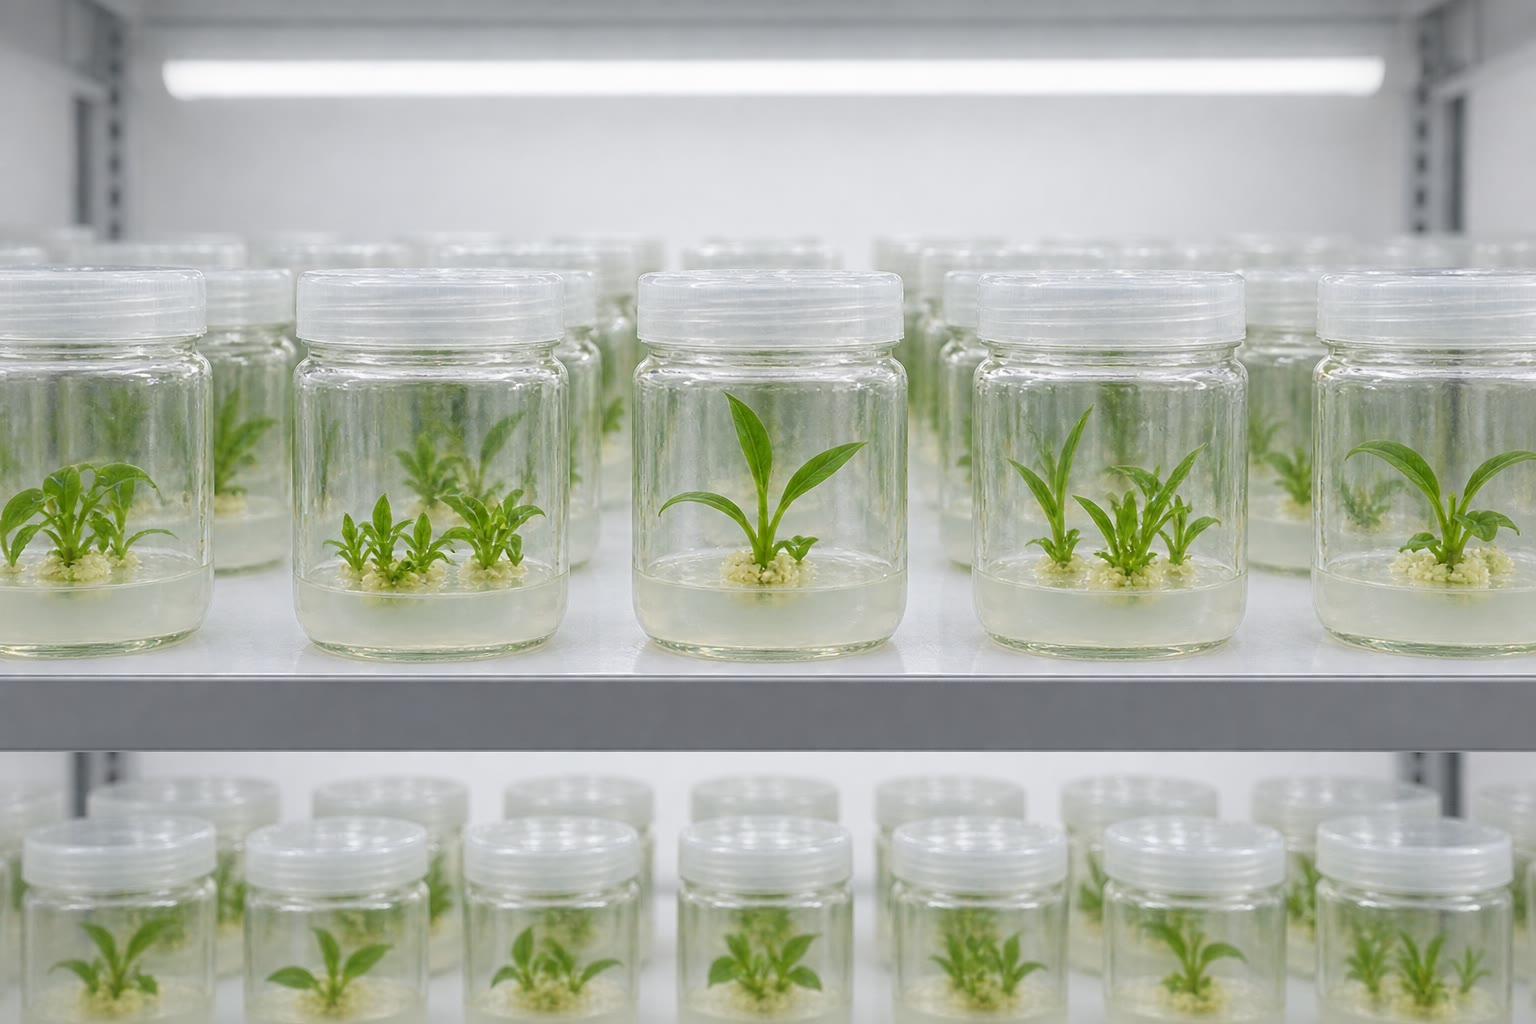
\includegraphics[width=0.6\linewidth]{images/book4/ai/b4-07-tissue-culture.jpg}

{\small نبيتات على آغار في غرفة إنماء: كل مرطبان يحوي \omterm{def:b2:asexual-reproduction:clone}{نسيلة} من
الصنف نفسه، مضاعفة من مرستيم واحد.}
\end{omfigure}

\section{كلفة الجنس وكلفة الاستغناء عنه}

\begin{theorem}[كلفة الجنس المضاعفة]\label{thm:b2:asexual-reproduction:twofold}
\index{كلفة الجنس المضاعفة}
في جمهرة تصنع كل أنثى فيها $F$ خلفًا، نصفهم أبناء، تضاعف أنثى طافرة
لاجنسية تصنع $F$ بنتًا، كلهن نسخ منها، نصيبَها من إناث الجيل التالي.
وإذا كان تواتر السلالة اللاجنسية $p$ بين الإناث،
كان في الجيل التالي
\[
p' = \frac{2p}{1 + p}, \qquad p_t = \frac{2^t p_0}{1 + (2^t - 1)p_0},
\]
أي إنها تبلغ من واحد في الألف نصفَ الجمهرة في
عشرة أجيال وكلَّها بعد ذلك بقليل. فالجنس، مع تساوي كل شيء آخر،
ينصّف معدل تكاثر السلالة --- وهو ثمن صنع الذكور. ولمّا كان الجنس
مع ذلك شبه كوني، لم يكن كل شيء آخر متساويًا: فعلى السلالات الجنسية
أن تكسب من إعادة التركيب، وسطيًا، عامل اثنين على الأقل.
\end{theorem}
\begin{proof}
عدد الإناث اللاجنسيات $pN$ ويخلّفن $FpN$ بنتًا؛ وعدد الإناث
الجنسيات $(1 - p)N$ ويخلّفن $F(1 - p)N/2$ بنتًا (والنصف
الآخر أبناء لا يصنعون بيوضًا). فنصيب اللاجنسيات من
البنات هو $Fp/(Fp + F(1 - p)/2) = 2p/(1 + p)$. وبكتابة $q = p/(1 -
p)$ يصير التكرار $q' = 2q$، ومنه $q_t = 2^t q_0$؛ وبالتحويل
رجوعًا نجد $p_t$. وبوضع $p_t = \tfrac12$ نجد $2^t q_0 = 1$، أي
$t = \log_2(1/q_0) \approx 10$ من أجل $p_0 = 10^{-3}$.
\end{proof}

\begin{omfigure}
\begin{tikzpicture}
\begin{axis}[
  width=0.76\linewidth, height=5.6cm,
  axis x line=bottom, axis y line=left,
  xmin=0, xmax=20, ymin=0, ymax=1.05,
  xlabel={الأجيال}, ylabel={تواتر السلالة اللاجنسية},
  xlabel style={font=\small, at={(axis description cs:0.5,-0.13)}, anchor=north},
  ylabel style={font=\small},
  tick label style={font=\small}, xtick={0,5,10,15,20}, ytick={0,0.5,1},
  legend style={font=\scriptsize, at={(0.5,-0.3)}, anchor=north, draw=none},
  clip=false,
]
\addplot[very thick, omThm, domain=0:20, samples=80] {2^x*0.001/(1+(2^x-1)*0.001)};
\addlegendentry{بلا فرق آخر: تستولي في 12 جيلًا}
\addplot[very thick, omDef, domain=0:20, samples=80] {0.001*(1.3)^x/(1+(1.3^x-1)*0.001)};
\addlegendentry{اللاجنسيات تخسر \qty{35}{\%} من اللياقة أمام الطفيليات: أبطأ}
\addplot[very thick, omProp, domain=0:20, samples=80] {0.001*(0.9)^x/(1+(0.9^x-1)*0.001)};
\addlegendentry{اللاجنسيات تخسر \qty{55}{\%}: لا تنتشر أبدًا}
\end{axis}
\end{tikzpicture}

{\small الميزة المضاعفة في العمل. انطلاقًا من واحد في الألف،
تستولي سلالة لاجنسية بلا أي مساوئ أخرى في اثني عشر جيلًا؛ ولا يكبحها
إلا غرم في اللياقة قدره النصف على الأقل --- من الطفيليات، أو
الطفرات المتراكمة، أو بطء التكيف.}
\end{omfigure}

\begin{proposition}[ما الغاية من الجنس]\label{prop:b2:asexual-reproduction:whysex}
\index{سقّاطة مولر}\index{فرضية الملكة الحمراء}
ثلاث فوائد كبيرة بما يكفي لتهم. \emph{\omterm{prop:b2:asexual-reproduction:whysex}{سقّاطة مولر}}:
ففي \omterm{def:b2:asexual-reproduction:clone}{النسيلة} يرث كل الخلف كل \omterm{def:b2:genome-diversification:mutation}{طفرة} ضارة، والمورثوم الخالي من
الطفرات، إذا ضاع مرة من جمهرة منتهية بالمصادفة، لا يمكن
إعادة صنعه أبدًا؛ فيرتفع العبء سقّاطةً، نقرة نقرة،
وتتحلل الجمهرات اللاجنسية الصغيرة. أما إعادة التركيب فتعيد بناء
مورثومات نظيفة من اثنين متأذيين. و\emph{التكيف}: فطفرتان نافعتان
تنشآن في فردين مختلفين من \omterm{def:b2:asexual-reproduction:clone}{نسيلة} تتنافسان
وتضيع إحداهما؛ أما في الجمهرة الجنسية فتجتمعان (فيشر ومولر،
في الثلاثينيات)، فتتكيف الجمهرات الجنسية أسرع حين يجب أن تتغير
مورّثات كثيرة. و\emph{الملكة الحمراء}: فالطفيليات تتكيف مع أشيع \omterm{def:b2:meiosis-heredity:vocabulary}{نمط
وراثي} عند المضيف، \omterm{def:b2:asexual-reproduction:clone}{والنسيلة}، وهي \omterm{def:b2:meiosis-heredity:vocabulary}{نمط وراثي} واحد، أشيع الجميع؛ أما
الأبوان الجنسيان فيصنعان من كل خلف قفلًا جديدًا. والحلزونات والأسماك
والنباتات التي لها جمهرات جنسية ونسيلية معًا تُظهر غلبة الجنسية حيث
تكثر الطفيليات. أما السلالات اللاجنسية المزدهرة --- الهندباء،
والدولابيات البدلوئيدية، ومعظم نسائل المحاصيل --- فهي إما حديثة،
أو هجن متعددة الصيغة تحمل تنوعها الخاص، أو يسندها مزارع يقتل
طفيلياتها عنها.
\end{proposition}

\begin{example}[زراعات أحادية من نسيلة]\label{ex:b2:asexual-reproduction:monoculture}
في أربعينيات القرن التاسع عشر كان معظم محصول البطاطا في إيرلندا
صنفًا نسيليًا واحدًا هو اللَّمبر؛ فلمّا وصل العفن المائي
\emph{Phytophthora infestans} سنة 1845، لقي بلدًا من نباتات
متطابقة وراثيًا قابلة للإصابة على السواء، فأتلف المحصول ثلاث سنوات
متتالية. وكان موز التصدير في العالم حتى الخمسينيات \omterm{def:b2:asexual-reproduction:clone}{نسيلة} واحدة هي
غرو ميشيل، فمُحيت من مزارع أمريكا الوسطى بفطر تربة؛ وبديلها،
كافنديش، \omterm{def:b2:asexual-reproduction:clone}{نسيلة} واحدة كذلك، وهي تُفقد اليوم، مزرعة بعد مزرعة، أمام
سلالة جديدة من الفطر نفسه، ولا تنوع لديها تقدمه في وجهها. \omterm{def:b2:asexual-reproduction:clone}{فالنسيلة}
أسهل هدف في الطبيعة، وعلى المزارع الذي يغرس \omterm{def:b2:asexual-reproduction:clone}{نسيلة} أن يوفّر المقاومة
التي كانت إعادة التركيب لتوفّرها مجانًا.
\end{example}

\section{تمارين}

\begin{exercise}[$\star$]\label{exo:b2:asexual-reproduction:1}
عرّف \omterm{def:b2:asexual-reproduction:clone}{النسيلة} \omterm{def:b2:asexual-reproduction:clone}{والجينيت} \omterm{def:b2:asexual-reproduction:clone}{والراميت}، وأعط ثلاثة أعضاء طبيعية \omterm{def:b2:asexual-reproduction:clone}{للتكاثر
الخضري} مع نبات لكل منها.
\end{exercise}

\begin{exercise}[$\star$]\label{exo:b2:asexual-reproduction:2}
في التطعيم، أي الأنسجة يجب أن تلتقي لينجح الاتحاد، وبماذا يسهم كل
شريك في الشجرة؟ ولماذا تكون الشجرة المطعّمة شيمرا لا هجينًا؟
\end{exercise}

\begin{exercise}[$\star$]\label{exo:b2:asexual-reproduction:3}
ميّز \omterm{def:b2:asexual-reproduction:apomixis}{التوالد العذري البذري} من \omterm{def:b2:asexual-reproduction:clone}{التكاثر الخضري}، \omterm{def:b2:asexual-reproduction:apomixis}{والتوالد العذري} من
كليهما. وأي الثلاثة يبقي \omterm{def:b2:angiosperm-reproduction:seed}{البذرة}؟
\end{exercise}

\begin{exercise}[$\star$]\label{exo:b2:asexual-reproduction:4}
اذكر خطوات \omterm{prop:b2:asexual-reproduction:tissueculture}{التكاثر المجهري} من المستنبت إلى النبات في الحقل، مسمّيًا
الشروط الهرمونية في كل خطوة.
\end{exercise}

\begin{exercise}[$\star\star$]\label{exo:b2:asexual-reproduction:5}
نبات فراولة يصنع 8 مدادات في السنة، ويجذّر كل منها 3
نبيتات، وكل نبيتة تفعل الشيء نفسه في السنة التالية.
فكم نباتًا بعد 4 سنوات إن لم يمت شيء؟ وعند \qty{0.1}{m^2} للنبات،
أي مساحة تلزمها؟ وما الذي يحد \omterm{def:b2:asexual-reproduction:clone}{النسيلة} فعلًا؟
\end{exercise}

\begin{exercise}[$\star\star$]\label{exo:b2:asexual-reproduction:6}
\omterm{def:b2:asexual-reproduction:clone}{لنسيلة} الحور باندو \num{47000} جذع على \qty{43}{ha}، ويعيش كل
جذع نحو \num{130} سنة. فإذا كان عمر \omterm{def:b2:asexual-reproduction:clone}{الجينيت} \num{14000} سنة،
فكم جيلًا من الجذوع مرّ عليه؟ واحسب متوسط تقدمه الشعاعي بالأمتار في
السنة، معاملًا إياه قرصًا.
\end{exercise}

\begin{exercise}[$\star\star$]\label{exo:b2:asexual-reproduction:7}
تنشأ طافرة لاجنسية بتواتر $10^{-4}$ في جمهرة جنسية، بالخصوبة
نفسها. احسب تواترها بعد 5 و10 و15 جيلًا. وكم يجب أن تنخفض
لياقتها لئلا تنتشر أبدًا؟
\end{exercise}

\begin{exercise}[$\star\star$]\label{exo:b2:asexual-reproduction:8}
تنبّأ بما يفعله دشبذ التبغ على أوساط نسبة الأوكسين إلى السيتوكينين
فيها 10 : 1 و1 : 1 و1 : 10، واشرح لماذا تُغمس عقلة الفرع في
أوكسين لا في سيتوكينين.
\end{exercise}

\begin{exercise}[$\star\star$]\label{exo:b2:asexual-reproduction:9}
تُزرع البطاطا درنات. والكيلوغرام المزروع يعطي
\qty{10}{kg}، والهكتار يحتاج إلى \qty{2}{t} من درنات البذار.
فانطلاقًا من \qty{1}{kg} من صنف جديد، كم موسمًا حتى يمكن زراعة
هكتار؟ ولماذا تعطي \omterm{def:b2:angiosperm-reproduction:seed}{البذرة} الحقيقية تكاثرًا أسرع ومع ذلك لا تُستعمل؟
\end{exercise}

\begin{exercise}[$\star\star\star$]\label{exo:b2:asexual-reproduction:10}
في جمهرة نسيلية من $N$ فردًا مع $U$ \omterm{def:b2:genome-diversification:mutation}{طفرة} ضارة
في المورثوم في الجيل، تكلف كل منها كسرًا $s$ من اللياقة،
يكون كسر الأفراد الخالين من الطفرات عند التوازن
$e^{-U/s}$ (وهو مشتق في \cref{ch:b2:population-genetics}). فمع $U =
0.1$ و$s = 0.02$، احسب عدد الأفراد الخالين من الطفرات
من أجل $N = 10^{5}$ ومن أجل $N = 10^{3}$، واشرح، \omterm{prop:b2:asexual-reproduction:whysex}{بسقّاطة
مولر}، لماذا تكون الجمهرة الصغيرة محكومًا عليها ولا تكون الكبيرة
كذلك --- بعد.
\end{exercise}

\begin{exercise}[$\star\star\star$]\label{exo:b2:asexual-reproduction:11}
تنشأ مرة واحدة سلالة ممرضة تتغلب على مقاومة \omterm{def:b2:meiosis-heredity:vocabulary}{نمط وراثي} معين.
قارن مصيرها في حقل من \omterm{def:b2:asexual-reproduction:clone}{نسيلة} واحدة وفي جمهرة جنسية تنفصل فيها
مورّثات المقاومة على عشرة مواقع، في كل منها أليلان متساويا
التواتر، واشرح مجاعة البطاطا الإيرلندية بهذه الألفاظ.
\end{exercise}

\begin{exercise}[$\star\star\star$]\label{exo:b2:asexual-reproduction:12}
«الجنس يكلف عامل اثنين وهو في كل مكان؛ واللاجنسية رخيصة
ونادرة.» ناقش تفسيرات الفصل الثلاثة، وقل ماذا تعني الدولابيات
البدلوئيدية --- اللاجنسية منذ أربعين مليون سنة --- في كل منها.
\end{exercise}

\section{مسألة: مزرعة فراولة ونسيلة قديمة}

\begin{problem}[{مسألة نهاية الأسبوع --- حساب النسيلة، من حقل
فراولة يملؤه المدادات ومختبر يضاعف مرستيمًا، إلى غزو جمهرة جنسية
بمتوالدة عذريًا والتحلل الوراثي لجينيت قديم، وتنتهي إلى زمن ملء
الحقل، وعدد النبيتات من مرستيم واحد، وتوازن المتوالدات عذريًا
والجنسيات}]
\label{pb:b2:asexual-reproduction:1}
يغرس مزارع \num{100} نبات فراولة في حقل مساحته
\qty{1}{ha} يحتمل \num{4} نباتات في المتر المربع. ويصنع كل
نبات \num{6} مدادات في السنة، يجذّر كل منها \num{2} بنتًا،
وتبقى النباتات كلها. ويضاعف مختبر الصنف نفسه بزرع
الأنسجة: فكل إعادة زراعة، كل \num{4} أسابيع، تضاعف
الفروع بعامل \num{5}؛ وينجو \qty{80}{\%} من النبيتات من الفطام.
وعقل الصنف العادية مصابة بالفيروس بنسبة \qty{90}{\%}؛
وقمم المرستيم البالغة \qty{0.3}{mm} تحمل الفيروس باحتمال
$0.02$. ومورثوم الحور: \qty{4.8e8}{} زوج أسس؛ \omterm{thm:b2:genome-diversification:rate}{ومعدل الطفر} الجسدي
\qty{1e-9}{} لكل زوج أسس في الانقسام الخلوي؛ و\num{20} انقسامًا
لخلايا المرستيم في السنة في فرع نامٍ.

\medskip
\noindent\textbf{الجزء الأول --- ملء الحقل.}
\begin{enumerate}
  \item كم نباتًا يحتمل الحقل؟
  \item بأي عامل يتضاعف عدد النباتات في كل سنة؟
  \item احسب عدد النباتات بعد 1 و2 و3 سنوات.
  \item حلّ $N(t) = 100\times 13^{t}$ لإيجاد الزمن الذي يمتلئ عنده
        الحقل.
  \item حين يمتلئ، لا تجد مكانًا إلا النباتات على حافة الرقعة.
        فإذا تقدمت الرقعة \qty{0.5}{m} في السنة، فكم سنة كان يلزم
        نباتًا واحدًا ليغطي الحقل بالتقدم وحده؟
  \item اشرح لماذا يغرس المزارع \num{100} نبات موزعة على الحقل
        بدل نبات واحد.
\end{enumerate}

\medskip
\noindent\textbf{الجزء الثاني --- المختبر.}
\begin{enumerate}[resume]
  \item كم إعادة زراعة تلزم للانتقال من مرستيم واحد إلى
        $10^{6}$ فرع على الأقل؟ وكم أسبوعًا؟
  \item كم نباتًا ينجو من الفطام؟
  \item ما احتمال أن يكون خط منحدر من مرستيم خاليًا من الفيروس؟
        وأن تكون الخطوط \num{10} المبدوءة من نبات واحد كلها كذلك؟
  \item يبدأ المختبر \num{10} خطوط ويتخلص من المصابة بعد اختبار.
        فما العدد المنتظر للخطوط النظيفة؟ وقارن ذلك بالعقل.
  \item اشرح لماذا تفلت قمة المرستيم من الفيروس.
  \item يمكن غرس الحقل من إنتاج المختبر في السنة الأولى بدل ملئه
        بالمدادات في ثلاث. أعط ميزة واحدة وخطرًا واحدًا لكل طريق.
\end{enumerate}

\medskip
\noindent\textbf{الجزء الثالث --- غزو متوالدة عذريًا.}
جمهرة هندباء جنسية؛ وتظهر فيها طافرة متوالدة عذريًا (تستنسخ البذور)
بتواتر $p_0 = 10^{-3}$ بإنتاج البذور نفسه لكل نبات.
ويذهب نصف الجهد التكاثري للنباتات الجنسية إلى \omterm{def:b2:plant-life-cycles:heterospory}{اللقاح}.
\begin{enumerate}[resume]
  \item برهن على التكرار $p' = 2p/(1 + p)$ لتواتر المتوالدة عذريًا
        بين أمهات البذور.
  \item احسب $p$ بعد 5 و10 أجيال، والجيل الذي تتجاوز عنده النصف.
  \item يتخصص فطر صدأ على أشيع \omterm{def:b2:meiosis-heredity:vocabulary}{نمط وراثي}: فينخفض إنتاج المتوالدة
        عذريًا من البذور بعامل $(1 - cp)$، مع
        $c = 0.8$. اكتب التكرار الجديد.
  \item أوجد تواتر التوازن $p^*$ وتحقق من استقراره
        من إشارة $p' - p$ على جانبيه.
  \item من أجل أي قيم $c$ تستولي المتوالدة عذريًا استيلاءً تامًا؟
  \item احسب التوازن من أجل $c = 0.6$. وفسّر: ماذا يجب على الطفيلي
        أن يفعل ليحمي الجنس؟
  \item المتوالدة عذريًا ثلاثية الصيغة. فلماذا لا تستطيع العودة إلى
        الجنس، ولماذا يهم هذا على المدى الطويل؟
\end{enumerate}

\medskip
\noindent\textbf{الجزء الرابع --- \omterm{def:b2:asexual-reproduction:clone}{النسيلة} القديمة.}
\begin{enumerate}[resume]
  \item احسب عدد الطفرات الجسدية في الانقسام الخلوي الواحد عند
        الحور.
  \item يفصل بين جذعين من \omterm{def:b2:asexual-reproduction:clone}{نسيلة} باندو \num{14000}
        سنة من النمو على كل جانب من سلفهما المشترك. فكم انقسامًا
        خلويًا يفصل بينهما، وكم \omterm{def:b2:genome-diversification:mutation}{طفرة} تميز مورثوميهما؟
  \item ما كسر المورثوم الذي يمثله ذلك؟ وإذا كانت \qty{2}{\%} من
        المورثوم مرمّزة، فكم فرقًا مرمّزًا؟
  \item لا \omterm{def:b2:meiosis-heredity:meiosis}{تقسم منصّف} في \omterm{def:b2:asexual-reproduction:clone}{النسيلة} ولا انتخاب على مستوى الكائن يزيل
        هذه الطفرات. فما الذي يزيلها، ولماذا يكون المنخل أضعف مما
        هو في سلالة جنسية؟
  \item هل باندو «موحدة وراثيًا»؟ ناقش في جملتين.
  \item اذكر النتيجة: زمن ملء الحقل بالمدادات، وعدد النبيتات التي
        يعطيها مرستيم واحد في سنة، وتواتر توازن المتوالدة عذريًا من
        أجل $c = 0.8$.
\end{enumerate}
\end{problem}
